\documentclass[conference]{IEEEtran}
\IEEEoverridecommandlockouts
\usepackage{cite}
\usepackage{balance}
\usepackage{amsmath,amssymb,amsfonts}
\usepackage{graphicx}
\usepackage{textcomp}
\usepackage{xcolor}
\usepackage{booktabs}
\usepackage{tikz}
\usetikzlibrary{positioning,arrows.meta,fit,calc}
\usepackage[hidelinks]{hyperref}
\newcommand{\NTrainGauges}{193}
\newcommand{\NGauges}{242}
\newcommand{\NTestGauges}{48}
\newcommand{\AblMinutes}{3.4}
\newcommand{\NTrainRows}{1,641,197}
\newcommand{\NValRows}{349,645}
\newcommand{\NTestRows}{52,994}
\newcommand{\PosRate}{5.5}
\newcommand{\NFeat}{50}
\newcommand{\Thr}{0.45}
\newcommand{\GroupFlow}{11}
\newcommand{\GroupRain}{10}
\newcommand{\GroupWeather}{5}
\newcommand{\GroupSoil}{6}
\newcommand{\GroupSeason}{2}
\newcommand{\GroupStatic}{16}
\newcommand{\XgbBA}{0.898}
\newcommand{\XgbPR}{0.737}
\newcommand{\XgbRec}{0.902}
\newcommand{\XgbPrec}{0.328}
\newcommand{\XgbBALo}{0.886}
\newcommand{\XgbBAHi}{0.910}
\newcommand{\PersBA}{0.750}
\newcommand{\PersPR}{0.428}
\newcommand{\PersRec}{0.508}
\newcommand{\PersPrec}{0.789}
\newcommand{\PersBALo}{0.724}
\newcommand{\PersBAHi}{0.778}
\newcommand{\ClimBA}{0.802}
\newcommand{\ClimPR}{0.203}
\newcommand{\ClimRec}{0.891}
\newcommand{\ClimPrec}{0.152}
\newcommand{\ClimBALo}{0.774}
\newcommand{\ClimBAHi}{0.829}
\newcommand{\LstmBA}{0.873}
\newcommand{\LstmPR}{0.589}
\newcommand{\LstmRec}{0.826}
\newcommand{\LstmPrec}{0.376}
\newcommand{\LstmBALo}{0.829}
\newcommand{\LstmBAHi}{0.911}
\newcommand{\NoFlowBA}{0.853}
\newcommand{\NoFlowPR}{0.494}
\newcommand{\NoFlowRec}{0.865}
\newcommand{\NoFlowPrec}{0.239}
\newcommand{\NoFlowBALo}{0.820}
\newcommand{\NoFlowBAHi}{0.880}
\newcommand{\DiffPersLo}{0.123}
\newcommand{\DiffPersHi}{0.175}
\newcommand{\LstmCov}{100}
\newcommand{\LstmCompare}{On the rows it covers, the model (0.898) and the simulation (0.873) were statistically indistinguishable in balanced accuracy, although only the model is a real forecast.}
\newcommand{\AblAllBA}{0.898}
\newcommand{\AblAllPR}{0.736}
\newcommand{\AlarmsThr}{150.2}
\newcommand{\PrecSeventyFive}{0.539}
\newcommand{\RecSeventyFive}{0.760}
\newcommand{\EceRaw}{0.102}
\newcommand{\EceIso}{0.005}
\newcommand{\CalWord}{over-confident}
\newcommand{\PgN}{46}
\newcommand{\PgMed}{0.900}
\newcommand{\PgQOne}{0.860}
\newcommand{\PgQThree}{0.926}
\newcommand{\PgMin}{0.769}
\newcommand{\EvN}{266}
\newcommand{\EvXgbWarn}{91.4}
\newcommand{\EvLstmWarn}{83.5}
\newcommand{\EvClimWarn}{89.5}
\newcommand{\EvPersWarn}{0.0}
\newcommand{\EvNoFlowWarn}{94.0}
\newcommand{\LeakRandBA}{0.915}
\newcommand{\LeakRandPR}{0.810}
\newcommand{\LeakTimeBA}{0.892}
\newcommand{\LeakTimePR}{0.724}
\newcommand{\LeakSpaceBA}{0.905}
\newcommand{\LeakSpacePR}{0.789}
\newcommand{\LeakSpTiBA}{0.898}
\newcommand{\LeakSpTiPR}{0.736}
\newcommand{\LeakGapBA}{1.7}
\newcommand{\LeakGapPR}{7.4}
\newcommand{\LeakText}{The random row split gave the highest balanced accuracy, 0.915, against 0.898 on unseen gauges in later years; the two bootstrap intervals (0.9115--0.9189 and 0.8862--0.9111) only just separate, and they come from different test sets, so the gap is indicative rather than tested. Random splitting inflated balanced accuracy by 1.7 points and PR-AUC by 7.4 points. PR-AUC ranged from 0.724 (new years) to 0.810 (random rows). Holding out later years lowered PR-AUC more than holding out gauges (0.724 against 0.789), although these are different test sets with different flood rates. In the spatial protocol, the test years are also the years from which each gauge's flood threshold was computed. Flood prevalence differs between protocols (7.4\% of random rows against 5.5\% in the held-out test), which moves PR-AUC on its own.}
\newcommand{\LeakDiscuss}{a refit scored on a random row split reached a balanced accuracy 1.7 points higher than the held-out protocol (Table~\ref{tab:leak}). The test sets and flood rates differ, so not all of this gap is leakage, but scores from random row splits should not be read as skill at a new gauge, and published Indian flood models can only be compared under the same split.}
\newcommand{\LeakConclude}{A random row split scored 1.7 points higher in balanced accuracy on its own test set.}
\newcommand{\LeakAbstract}{A refit scored on a random row split reached 0.915, 1.7 points higher on its own test set.}
\newcommand{\LeadOne}{96.7}
\newcommand{\LeadOneRise}{90.3}
\newcommand{\LeadTwo}{93.3}
\newcommand{\LeadTwoRise}{85.2}
\newcommand{\LeadThree}{89.5}
\newcommand{\LeadThreeRise}{80.0}
\newcommand{\FpMonsoonPct}{86}
\newcommand{\MonPrec}{0.311}
\newcommand{\OthPrec}{0.415}
\newcommand{\MonAlarms}{372}
\newcommand{\OthAlarms}{36}
\newcommand{\NearMissMon}{21}
\newcommand{\FaRatioMon}{41}
\newcommand{\PgGauges}{46}
\newcommand{\RhoArea}{0.44}
\newcommand{\PArea}{0.002}
\newcommand{\PMinOther}{0.64}
\newcommand{\WarnThreeXgb}{63.9}
\newcommand{\WarnThreeLstm}{78.9}
\newcommand{\WarnThreeClim}{89.1}
\newcommand{\EvGauges}{44}
\newcommand{\MeanLeadXgb}{2.58}
\newcommand{\ImpFlow}{67.5}
\newcommand{\ImpRain}{13.6}
\newcommand{\ImpWeather}{7.3}
\newcommand{\ImpTopOne}{40.5}
\newcommand{\ImpTopTwo}{23.9}
\newcommand{\ImpRainDay}{8.5}
\newcommand{\RelHiConf}{0.97}
\newcommand{\RelHiFreq}{0.75}
\newcommand{\OnsetAll}{0.852}
\newcommand{\OnsetNoFlow}{0.846}
\newcommand{\OnsetFlowOnly}{0.810}
\newcommand{\AblOnMaxDelta}{0.0051}
\newcommand{\OnXgbBA}{0.857}
\newcommand{\OnXgbPR}{0.369}
\newcommand{\OnLstmBA}{0.877}
\newcommand{\OnLstmPR}{0.421}
\newcommand{\OnTrendBA}{0.734}
\newcommand{\OnTrendPR}{0.158}
\newcommand{\OnClimBA}{0.802}
\newcommand{\OnClimPR}{0.102}
\newcommand{\OnPersBA}{0.500}
\newcommand{\OnPersPR}{0.026}
\newcommand{\TrendBA}{0.828}
\newcommand{\TrendPR}{0.605}
\newcommand{\LstmDiffLo}{-0.009}
\newcommand{\LstmDiffHi}{0.063}
\newcommand{\LstmDiffOnLo}{-0.045}
\newcommand{\LstmDiffOnHi}{0.011}
\newcommand{\LstmAlarm}{120}
\newcommand{\MatchPrec}{0.394}
\newcommand{\MatchRec}{0.864}
\newcommand{\UnseenNoRows}{1}
\newcommand{\SeenTestGauges}{181}
\newcommand{\NUnseenGauges}{49}
\newcommand{\BrierRaw}{0.065}
\newcommand{\BrierIso}{0.025}
\newcommand{\BrierClim}{0.048}
\newcommand{\EceRawLo}{0.094}
\newcommand{\EceRawHi}{0.110}
\newcommand{\EceIsoLo}{0.002}
\newcommand{\EceIsoHi}{0.008}
\newcommand{\EceMonRaw}{0.250}
\newcommand{\EceMonIso}{0.014}
\newcommand{\EceOthRaw}{0.026}
\newcommand{\YearMinBA}{0.873}
\newcommand{\YearMaxBA}{0.914}
\newcommand{\YearMin}{2017}
\newcommand{\YearMax}{2016}
\newcommand{\YearsBig}{2015--2018}
\newcommand{\YearsSmallRows}{2,102}
\newcommand{\YearsSmall}{2019 and 2020}
\newcommand{\YearsSmallBA}{0.783 and 0.767}
\newcommand{\RegRho}{0.37}
\newcommand{\RegP}{0.02}
\newcommand{\RegRhoRes}{0.20}
\newcommand{\RegPRes}{0.23}
\newcommand{\RegDams}{37}
\newcommand{\RegNoDams}{9}
\newcommand{\RegBADams}{0.911}
\newcommand{\RegBANoDams}{0.875}
\newcommand{\NsTrain}{5.0}
\newcommand{\NsTest}{3.9}
\newcommand{\DropN}{281,360}
\newcommand{\DropPct}{9.3}
\newcommand{\DropMon}{26}
\newcommand{\KeptMon}{34}
\newcommand{\DropHigh}{1.5}
\newcommand{\KeptHigh}{4.9}
\newcommand{\EpN}{1,441}
\newcommand{\EpFalse}{1,106}
\newcommand{\EpFalsePct}{77}
\newcommand{\RandWarn}{38.6}
\newcommand{\RandWarnMon}{75.2}
\newcommand{\SplitN}{5}
\newcommand{\SplitBAMin}{0.877}
\newcommand{\SplitBAMax}{0.898}
\newcommand{\SplitPRMin}{0.706}
\newcommand{\SplitPRMax}{0.764}
\newcommand{\SplitOnMin}{0.822}
\newcommand{\SplitOnMax}{0.851}
\newcommand{\SplitGainMin}{0.119}
\newcommand{\SplitGainMax}{0.136}
\newcommand{\BasinN}{5}
\newcommand{\BasinCount}{15}
\newcommand{\BasinOnMin}{0.785}
\newcommand{\BasinOnMax}{0.864}
\newcommand{\BasinWorst}{Cauvery, EFRN, EFRS, Tapi}
\newcommand{\BasinBAMin}{0.866}
\newcommand{\BasinBAMax}{0.906}
\newcommand{\BasinPRMin}{0.648}
\newcommand{\BasinPRMax}{0.829}
\newcommand{\BasinGainMin}{0.094}
\newcommand{\BasinGainMax}{0.186}
\newcommand{\BasinPersMin}{0.699}
\newcommand{\BasinPersMax}{0.812}
\newcommand{\BasinBelowSplits}{2}
\newcommand{\MetBA}{0.832}
\newcommand{\MetOnBA}{0.825}
\newcommand{\MetPR}{0.447}
\newcommand{\QnnBA}{0.853}
\newcommand{\QnnPR}{0.364}
\newcommand{\QnnPrev}{1.6}
\newcommand{\QnnPrec}{0.117}
\newcommand{\QnnOnBA}{0.798}
\newcommand{\NcwEce}{0.008}
\newcommand{\NcwBA}{0.902}
\newcommand{\NcwText}{A refit without the positive-class weight, run after the test results were known, had a raw ECE of 0.008 at a balanced accuracy of 0.902 (onset 0.863), against 0.898 and 0.852 for the same sample with the weight. The weighting therefore caused most of the over-confidence and bought no skill; the monsoon gap in ECE reflects where the high scores fall.}
\newcommand{\CandLrBA}{0.899}
\newcommand{\CandLrPR}{0.751}
\newcommand{\CandSelBA}{0.911}
\newcommand{\CandSelPR}{0.796}
\newcommand{\CandGainPR}{4.5}


\begin{document}

\title{Forecasting Three-Day High-Flow Exceedance at\\
Gauges Unseen in Space and Time: A Leakage-Controlled\\
Benchmark on CAMELS-IND}

\author{\IEEEauthorblockN{Anonymous Author(s)}
\IEEEauthorblockA{\textit{Affiliation withheld for double-blind review}}}

\maketitle

\begin{abstract}
Flood warnings in India are issued gauge by gauge, yet machine-learning flood forecasters are often scored on random row splits that let neighbouring days of the same river leak between training and test data. We build a leakage-controlled benchmark on CAMELS-IND for one operational question: will a gauge's flow reach its 95th-percentile level, a high-flow proxy for a flood level exceeded on about 18 days a year, within the next three days? We train on \NTrainGauges{} gauges for 1980--2008, select models and thresholds on 2009--2014, and test on \NTestGauges{} unseen gauges in 2015--2020. A gradient-boosted model reached a balanced accuracy of \XgbBA{} (95\% gauge-bootstrap interval \XgbBALo--\XgbBAHi) and a PR-AUC of \XgbPR, above persistence and gauge climatology, and not significantly different from the dataset's regional LSTM simulation (\LstmBA), which is driven by observed future rain and was trained on years that overlap ours in 2015. On days when the river was still below the level, where a warning matters, balanced accuracy was \OnXgbBA{} and recall fell from \LeadOneRise\% one day ahead to \LeadThreeRise\% three days ahead (\LeadOne\% to \LeadThree\% over all flood days), again not significantly different from the LSTM. \LeakAbstract{} Five other gauge splits gave \SplitBAMin--\SplitBAMax{} and leave-basin-out folds \BasinBAMin--\BasinBAMax. Precision was \XgbPrec, with most false alarms in the monsoon, so a positive forecast should trigger review by an officer.
\end{abstract}

\begin{IEEEkeywords}
CAMELS-IND, data leakage, flood forecasting, gradient boosting, hydrological benchmark
\end{IEEEkeywords}

\section{Introduction}
Indian flood warnings are issued per gauge, and an emergency officer needs to know whether the flow is likely to reach its flood level in the next few days. Models trained on many catchments now simulate streamflow well, even in ungauged basins \cite{Kratzert2019a,Kratzert2019b,Nearing2024}. Reported skill, however, depends on how a model is evaluated. When rows are split at random, days from the same flood fall on both sides of the split, and part of the test score then rewards memory of the event \cite{Kapoor2023,Roberts2017}.

For India, CAMELS-IND provides daily forcing, observed streamflow and catchment attributes for peninsular Indian catchments \cite{Mangukiya2025}, in the format of the CAMELS family \cite{Newman2015,Addor2017}. It also ships a regional LSTM streamflow simulation, a strong deep-learning reference. No short-range flood-exceedance benchmark on these gauges yet controls leakage, compares against simple and strong references, and reports the numbers an operations room needs: alarm rates, onset lead time and calibration.

Our contributions are:
\begin{enumerate}
\item A leakage-controlled task and split: gauges held out in space and time, flood thresholds from training years only, model and threshold selection on validation only, and one scoring of the selected model on the test set; later test-set diagnostics are marked post hoc (Fig.~\ref{fig:split}).
\item A measurement of how much the evaluation protocol changes the score: one model configuration scored under random, temporal, spatial and space-and-time splits.
\item A comparison with persistence, the gauge's own climatology and the CAMELS-IND regional LSTM simulation, with gauge-cluster bootstrap intervals.
\item A feature-group ablation that shows what the forecast relies on, including a variant that needs no streamflow reading at forecast time.
\item An operational analysis of operating points, calibration, per-gauge skill and the lead time of warnings before flood onsets.
\end{enumerate}

\section{Related Work}
\textit{Large-sample learning.} The CAMELS datasets standardised forcing, flow and attributes across hundreds of basins \cite{Newman2015,Addor2017}. LSTMs trained on them learn regional behaviour \cite{Kratzert2019a}, predict ungauged basins \cite{Kratzert2019b} and simulate extremes better than conceptual models \cite{Frame2022}; at global scale, a learned model forecasts extreme floods in ungauged watersheds with skill comparable to an operational system \cite{Nearing2024}. Graph models that encode the river network have so far not beaten models that ignore it \cite{Kirschstein2024}. Most of this work simulates streamflow; flood \emph{exceedance}, the quantity a warning is issued on, is usually derived afterwards.

\textit{Operational forecasting.} Physically based ensemble systems such as GloFAS \cite{Alfieri2013} dominate operational flood forecasting \cite{Cloke2009}. Machine learning has also reached operations: a system run for India and Bangladesh combines learned river-stage forecasts with inundation models \cite{Nevo2022}. In India, the INDOFLOODS catalogue documents historical events \cite{Kuntla2025} and many studies apply tree ensembles or neural networks to single basins \cite{Mosavi2018}, often with random splits.

\textit{Evaluation.} Leakage through the split is a leading cause of irreproducible machine-learning results \cite{Kapoor2023}, and data with spatial or temporal structure need blocked validation \cite{Roberts2017}. For rare events, precision--recall curves are more informative than ROC curves \cite{Saito2015}, and probabilistic forecasts should be checked for calibration \cite{Brier1950}.

To our knowledge, no study has benchmarked short-range flood-exceedance forecasting on CAMELS-IND with a space-and-time held-out split against both a learned streamflow simulation and simple references.


\section{Data and Task}
\subsection{Target}
For gauge $g$ on day $t$ the target is
\begin{equation}
y_{g,t}=\mathbb{1}\Big[\max_{h\in\{1,2,3\}} Q_{g,t+h}\ \ge\ q^{95}_g\Big],
\label{eq:target}
\end{equation}
where $Q$ is observed streamflow and $q^{95}_g$ is the 95th percentile of the gauge's flow over the training years 1980--2008 only. A day with $y_{g,t}=1$ is a \emph{flood window}. The level is a statistical proxy, exceeded on about 18 days a year, not an official danger level, which CAMELS-IND does not provide; a stricter 99th-percentile level is tested in Section~\ref{sec:robust}. A three-day horizon matches the time an officer needs to stage teams. Days without a flow observation in the horizon are dropped: \DropN{} gauge-days (\DropPct\% of the observed spans). They were not concentrated in floods: \DropMon\% fell in the monsoon against \KeptMon\% of the kept days, and \DropHigh\% followed a day at or above $q^{95}_g$ against \KeptHigh\%.

\subsection{Inputs}
Table~\ref{tab:feat} lists the \NFeat{} inputs, all known at the end of day $t$. Flow features are scaled by $q^{95}_g$, so they read as ``how close the river is to its flood level''. Hydrological signatures of CAMELS-IND are excluded, because they are computed over the full 1980--2020 record and would leak test-period information; future rainfall is excluded as well. Rainfall is IMD's gridded product and soil moisture, humidity and evapotranspiration come from the IMDAA reanalysis and GLEAM \cite{Mangukiya2025}; these are available with a delay, so in real time they would be replaced by forecasts or near-real-time estimates, and the skill reported here is an upper bound for that setting.

\begin{table}[t]
\caption{Input groups (all known at the end of day $t$)}
\label{tab:feat}
\centering
\footnotesize
\setlength{\tabcolsep}{3pt}
\begin{tabular}{llc}
\toprule
Group & Content & Inputs\\
\midrule
Streamflow & lags 0--3, changes, 7/30-day means and maxima & \GroupFlow\\
Rainfall & lags 0--3, 3--90-day sums, 7-day maximum & \GroupRain\\
Weather & temperature, humidity, evapotranspiration & \GroupWeather\\
Soil moisture & four layers and recent changes & \GroupSoil\\
Season & day of year (sine, cosine) & \GroupSeason\\
Catchment & area, slope, aridity, land cover, soils & \GroupStatic\\
\bottomrule
\end{tabular}
\end{table}

\subsection{Split}
Fig.~\ref{fig:split} shows the split. All \NGauges{} gauges in the streamflow file have forcing data and at least three years of flow in 1980--2008. The data description counts 228 catchments with more than 30\% flow availability \cite{Mangukiya2025}, but all \NGauges{} gauges of the version we use pass that filter, so none is excluded. A group split puts 20\% of gauges aside (seed 42), so the primary test asks about rivers the model has never seen, in years it has never seen; one of the \NUnseenGauges{} unseen gauges has no flow record in 2015--2020, which leaves \NTestGauges{} test gauges. Training uses the other gauges in 1980--2008 (\NTrainRows{} gauge-days), validation the same gauges in 2009--2014 (\NValRows), and the test the unseen gauges in 2015--2020, all labelled by (\ref{eq:target}) (\NTestRows{} gauge-days, of which \PosRate\% are flood windows).

\begin{figure}[t]
\centering
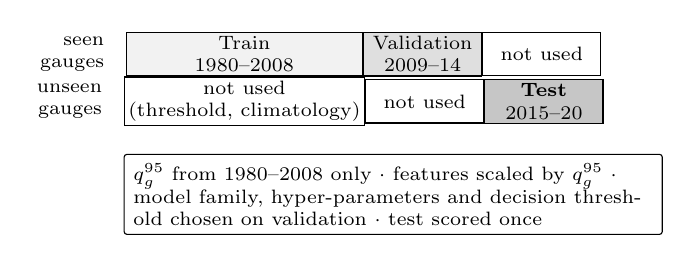
\begin{tikzpicture}[font=\scriptsize,
  cell/.style={draw, minimum height=0.55cm, align=center, inner sep=1.5pt},
  arr/.style={-{Latex[length=1.4mm]}, semithick}]
\node[cell, minimum width=3.0cm, fill=gray!10] (tr) at (0,0) {Train\\1980--2008};
\node[cell, minimum width=1.5cm, fill=gray!25, right=0pt of tr] (va) {Validation\\2009--14};
\node[cell, minimum width=1.5cm, right=0pt of va] (sx) {not used};
\node[cell, minimum width=3.0cm, below=0pt of tr] (ux) {not used\\(threshold, climatology)};
\node[cell, minimum width=1.5cm, right=0pt of ux] (uy) {not used};
\node[cell, minimum width=1.5cm, fill=gray!45, right=0pt of uy] (te) {\textbf{Test}\\2015--20};
\node[left=0.15cm of tr, align=right] {seen\\gauges};
\node[left=0.15cm of ux, align=right] {unseen\\gauges};
\node[draw, rounded corners=1pt, align=left, below=0.35cm of ux.south west, anchor=north west, text width=6.6cm] (rules)
 {$q^{95}_g$ from 1980--2008 only $\cdot$ features scaled by $q^{95}_g$ $\cdot$ model family, hyper-parameters and decision threshold chosen on validation $\cdot$ test scored once};
\end{tikzpicture}
\caption{Leakage-controlled split. The primary test uses gauges and years that played no part in training, model selection or threshold choice. The unseen gauges' 1980--2008 record is used only to set their flood threshold and climatology.}
\label{fig:split}
\end{figure}

\section{Methods}
\textit{Model.} Six candidates (logistic regression, random forest, histogram gradient boosting and XGBoost \cite{Chen2016} at three depths) and a refit of the depth-6 model were compared on validation balanced accuracy (Table~\ref{tab:cand}), and the decision threshold of the selected depth-6 XGBoost model, \Thr, was set on validation as well. It uses a learning rate of 0.05, subsampling of rows and columns at 0.8, a minimum child weight of 20, L2 regularisation of 5, a positive-class weight equal to the ratio of negative to positive training rows, and early stopping on validation PR-AUC, and it was refit on all training rows. Logistic regression reached a validation balanced accuracy of \CandLrBA{} against \CandSelBA{} for the selected model, so the selected refit adds little balanced accuracy but \CandGainPR{} points of PR-AUC. With $\mathrm{TPR}$ and $\mathrm{TNR}$ the true positive and true negative rates,
\begin{equation}
\mathrm{BA}=\tfrac12\left(\mathrm{TPR}+\mathrm{TNR}\right).
\label{eq:ba}
\end{equation}

\begin{table}[t]
\caption{Candidate models on validation (seen gauges, 2009--2014)}
\label{tab:cand}
\centering
\footnotesize
\begin{tabular}{lcc}
\toprule
Model & BA & PR-AUC\\
\midrule
Logistic regression & 0.899 & 0.751\\
Random forest & 0.905 & 0.781\\
Hist. gradient boosting & 0.909 & 0.791\\
XGBoost, depth 4 & 0.909 & 0.790\\
XGBoost, depth 6 & 0.909 & 0.792\\
XGBoost, depth 8 & 0.909 & 0.793\\
XGBoost, depth 6, selected refit & 0.911 & 0.796\\
\bottomrule
\end{tabular}
\end{table}

\textit{References.} \emph{Persistence} forecasts a flood window if the river is above its flood level today. A \emph{trend rule} needs no learning: its score is $Q_{g,t}/q^{95}_g+\max(0,Q_{g,t}-Q_{g,t-3})/q^{95}_g$, so a high or rising river raises an alarm. \emph{Climatology} forecasts the gauge's own 1980--2008 rate of flood windows within $\pm15$ days of the calendar day. The \emph{LSTM simulation} is the regional LSTM streamflow of CAMELS-IND \cite{Mangukiya2025}, scored as $\max_{h\le3}\hat Q_{g,t+h}/q^{95}_g$. It is driven by observed forcing, so it sees the rain of days $t{+}1$ to $t{+}3$, which no real forecast has. It was trained by the dataset authors on 159 catchments over 1991--2015 and tested on 2016--2020 \cite{Mangukiya2025}, so it has most likely seen our test gauges and, in 2015, one of our test years; it is an optimistic reference, not a held-out competitor. Thresholds of the references were set on validation like the model's.

\textit{Analyses.} We refit the selected configuration on the same 500,000-row training sample with one input group removed at a time, and with the streamflow and season inputs only. Confidence intervals come from 1,000 resamples of the test gauges, which keeps each river's days together. Calibration is the expected calibration error over ten bins, before and after isotonic regression fitted on validation. A flood onset is a day on which the river reaches $q^{95}_g$ after at least seven days below it; a method warns of it if it forecasts a flood window one, two or three days earlier. For lead-day and seasonal analyses, a flood day at lead $h$ is a day $t$ with $Q_{g,t+h}\ge q^{95}_g$, and the monsoon is June to September. Sensitivity refits (Section~\ref{sec:robust}) use the ablation's 500,000-row sample: five more random gauge splits (seeds 1 to 5), a leave-basin-out evaluation in which the CAMELS-IND river basins are grouped into five folds and every basin is held out once, and the same task with the 99th percentile as level.

\textit{Reproducibility.} The primary split and the bootstrap use seed 42, and the \NUnseenGauges{} held-out gauges are stored with the model metadata; code, model and split lists will be released after review. Re-scoring the stored model reproduces its recorded test balanced accuracy exactly, and every number in this paper is generated from the experiment outputs by a script that also checks each claim made about it.

\section{Results}
\subsection{Skill on Unseen Gauges}
Table~\ref{tab:main} and Fig.~\ref{fig:pr} give the main comparison, with balanced accuracy as defined in (\ref{eq:ba}). The model scored above persistence and climatology in balanced accuracy and PR-AUC, and its bootstrap interval for the gain in balanced accuracy over persistence (\DiffPersLo--\DiffPersHi) excludes zero. Persistence was more precise (\PersPrec{} against \XgbPrec) but misses every flood that has not yet begun. The model's recall of \XgbRec{} means that it found nine in ten flood windows at rivers it had never seen. Many of these windows are easy: a river above its level usually stays there. On onset rows, where the river is still below the level, the model's balanced accuracy was \OnXgbBA{} and its PR-AUC \OnXgbPR, against \OnTrendBA{} and \OnTrendPR{} for the trend rule, \OnClimBA{} and \OnClimPR{} for climatology and \OnPersBA{} for persistence, which cannot anticipate an onset.

\begin{table}[t]
\caption{Three-day exceedance on \NTestGauges{} unseen gauges, 2015--2020}
\label{tab:main}
\centering
\footnotesize
\setlength{\tabcolsep}{1.3pt}
\begin{tabular}{lccccccc}
\toprule
 & \multicolumn{5}{c}{all rows} & \multicolumn{2}{c}{onset rows}\\
Method & BA & 95\% CI & PR-AUC & Rec. & Prec. & BA & PR-AUC\\
\midrule
XGBoost (ours) & 0.898 & 0.886--0.910 & 0.737 & 0.902 & 0.328 & 0.857 & 0.369\\
No-flow XGB. & 0.853 & 0.820--0.880 & 0.494 & 0.865 & 0.239 & 0.846 & 0.257\\
LSTM sim.$^\dagger$ & 0.873 & 0.829--0.911 & 0.589 & 0.826 & 0.376 & 0.877 & 0.421\\
Trend rule & 0.828 & -- & 0.605 & 0.754 & 0.305 & 0.734 & 0.158\\
Climatology & 0.802 & 0.774--0.829 & 0.203 & 0.891 & 0.152 & 0.802 & 0.102\\
Persistence & 0.750 & 0.724--0.778 & 0.428 & 0.508 & 0.789 & 0.500 & 0.026\\
\bottomrule
\multicolumn{8}{l}{\scriptsize CI: gauge-cluster bootstrap. Onset rows: river below $q^{95}_g$ on day $t$.}\\
\multicolumn{8}{l}{\scriptsize $^\dagger$Driven by observed future rain; covers every test row.}\\
\end{tabular}
\end{table}

\begin{figure}[t]
\centering
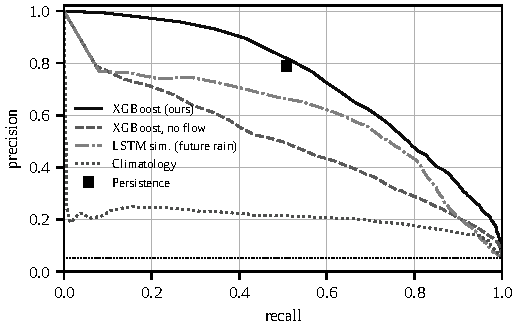
\includegraphics[width=0.9\columnwidth]{fig_pr.pdf}
\caption{Precision--recall curves on the unseen test gauges. The square is persistence; the dotted line is the flood rate.}
\label{fig:pr}
\end{figure}

The LSTM simulation is a demanding reference because it knows the rain that is still to fall. Over all rows its balanced accuracy was \LstmBA{} against \XgbBA{} for the model, and the paired gauge-bootstrap interval of the difference, \LstmDiffLo{} to \LstmDiffHi, includes zero. The two also run at different operating points: at the LSTM's alarm rate (\LstmAlarm{} per 1,000 gauge-days) the model reached a precision of \MatchPrec{} and a recall of \MatchRec, against \LstmPrec{} and \LstmRec. On onset rows the LSTM scored higher (\OnLstmBA{} against \OnXgbBA), as its access to future rain would suggest, but the difference interval (\LstmDiffOnLo{} to \LstmDiffOnHi) includes zero.

\subsection{Effect of the Evaluation Protocol}
To measure what the split itself does to the score, we trained the same configuration on a 500,000-row sample under four protocols, each with its own validation set for early stopping and threshold, and scored it once (Table~\ref{tab:leak}). \LeakText{}

\begin{table}[t]
\caption{Same configuration, four protocols (500,000-row refit)}
\label{tab:leak}
\centering
\footnotesize
\setlength{\tabcolsep}{1.4pt}
\begin{tabular}{lcccccc}
\toprule
Test set & Gauges & Flood \% & BA & 95\% CI & PR-AUC & Prec.\\
\midrule
Random rows & 242 & 7.4 & 0.915 & 0.911--0.919 & 0.810 & 0.426\\
New years & 181 & 6.1 & 0.892 & 0.885--0.898 & 0.724 & 0.349\\
New gauges & 49 & 7.6 & 0.905 & 0.898--0.912 & 0.789 & 0.424\\
New gauges and years & 48 & 5.5 & 0.898 & 0.886--0.911 & 0.736 & 0.340\\
\bottomrule
\multicolumn{7}{l}{\scriptsize Random: 70/10/20\% of gauge-days; others trained on seen gauges, 1980--2008.}\\
\multicolumn{7}{l}{\scriptsize New years: seen gauges, 2015--20. New gauges: unseen, 1980--2008.}\\
\end{tabular}
\end{table}

\subsection{What the Forecast Relies On}
Table~\ref{tab:abl} shows the ablation. Over all rows, removing the streamflow inputs cost the most, lowering balanced accuracy from \AblAllBA{} to \NoFlowBA{} and PR-AUC from \AblAllPR{} to \NoFlowPR, while removing soil moisture, rainfall or catchment attributes cost little. Much of that score comes from rivers that are already high and stay high. On onset rows, where the river is still below its flood level, removing streamflow lowered onset balanced accuracy only from \OnsetAll{} to \OnsetNoFlow, streamflow and season alone reached \OnsetFlowOnly{} and meteorology and season alone \MetOnBA. The two kinds of input are complementary for onsets, and neither alone reaches the full model. Within the meteorological inputs the groups are redundant: removing rainfall, soil moisture or catchment attributes one at a time changed onset balanced accuracy by at most \AblOnMaxDelta{} (each removal raised it slightly), so these single-group results cannot rank them. The no-flow variant also scored above climatology overall (\NoFlowBA{} against \ClimBA, with overlapping intervals), so it is a possible fallback when a gauge reading is missing.

The selected model's gain importance agrees: streamflow inputs account for \ImpFlow\% of the total gain, led by today's flow relative to the flood level (\ImpTopOne\%) and its seven-day maximum (\ImpTopTwo\%), followed by rainfall (\ImpRain\%, of which today's rain alone \ImpRainDay\%). Gain importance favours inputs used in many splits, so we use it only as a check on the ablation.


\begin{table}[t]
\caption{Feature-group ablation (same 500k training sample)}
\label{tab:abl}
\centering
\footnotesize
\setlength{\tabcolsep}{3pt}
\begin{tabular}{lccccc}
\toprule
Inputs & $n$ & BA & PR-AUC & Rec. & Onset BA\\
\midrule
All inputs & 50 & 0.898 & 0.736 & 0.897 & 0.852\\
No streamflow & 39 & 0.853 & 0.494 & 0.865 & 0.846\\
No catchment & 34 & 0.895 & 0.734 & 0.907 & 0.855\\
No soil moisture & 44 & 0.896 & 0.732 & 0.895 & 0.854\\
No rainfall & 40 & 0.897 & 0.730 & 0.901 & 0.857\\
Streamflow + season & 13 & 0.875 & 0.685 & 0.882 & 0.810\\
\bottomrule
\multicolumn{6}{l}{\scriptsize Onset BA: rows where the river is below its flood level on day $t$.}\\
\end{tabular}
\end{table}

\subsection{Sensitivity to Split and Level}
\label{sec:robust}
Table~\ref{tab:robust} repeats the evaluation under other splits and a stricter level. Over five more random gauge splits the balanced accuracy ranged from \SplitBAMin{} to \SplitBAMax{} and the onset balanced accuracy from \SplitOnMin{} to \SplitOnMax, so the primary refit (\AblAllBA) lies at the top of that range. Holding out whole river basins gave \BasinBAMin--\BasinBAMax{} (onset \BasinOnMin--\BasinOnMax), below every random split in \BasinBelowSplits{} folds, but persistence also varied across folds (\BasinPersMin--\BasinPersMax): the gain over persistence was \SplitGainMin--\SplitGainMax{} over the random splits and \BasinGainMin--\BasinGainMax{} over the basin folds. With the 99th percentile as level (\QnnPrev\% of test rows positive) the balanced accuracy was \QnnBA{} and the PR-AUC \QnnPR{} at a precision of \QnnPrec. Skill per test year ranged from \YearMinBA{} (\YearMin) to \YearMaxBA{} (\YearMax) over \YearsBig; \YearsSmall{} have only \YearsSmallRows{} gauge-days in the dataset. Gauges with dams upstream scored higher than those without (median per-gauge balanced accuracy \RegBADams{} for \RegDams{} gauges against \RegBANoDams{} for \RegNoDams; Spearman $\rho=\RegRho$ with the number of dams, $p=\RegP$, but $\rho=\RegRhoRes$, $p=\RegPRes$ with the reservoir index); these attribute tests were not corrected for multiple comparisons. The level was also exceeded less often in the test years (\NsTest\% of days) than in the training years that defined it (\NsTrain\%).

\begin{table}[t]
\caption{Sensitivity refits (500,000-row training sample)}
\label{tab:robust}
\centering
\footnotesize
\setlength{\tabcolsep}{1.8pt}
\begin{tabular}{lcccc}
\toprule
Evaluation & Test gauges & BA & PR-AUC & Onset BA\\
\midrule
5 gauge splits & range & 0.877--0.898 & 0.706--0.764 & 0.822--0.851\\
5 basin folds & range & 0.866--0.906 & 0.648--0.829 & 0.785--0.864\\
99th pct.\ level & 48 & 0.853 & 0.364 & 0.798\\
met.\ + season only & 48 & 0.832 & 0.447 & 0.825\\
no class weight & 48 & 0.902 & 0.737 & 0.863\\
\bottomrule
\end{tabular}
\end{table}

\subsection{Operational Behaviour}
Precision is the main weakness. At the validation threshold the model raised \AlarmsThr{} alarms per 1,000 gauge-days at a precision of \XgbPrec{} (Table~\ref{tab:ops}); raising the threshold to 0.75 halved the alarms and lifted precision to \PrecSeventyFive, at a recall of \RecSeventyFive. Because a positive forecast in our system leads to human review rather than automatic action, the validation threshold is a reasonable default. The raw probabilities were \CalWord{} (ECE \EceRaw, gauge-bootstrap interval \EceRawLo--\EceRawHi; Brier score \BrierRaw, worse than climatology's \BrierClim); isotonic recalibration on validation data lowered the ECE to \EceIso{} (\EceIsoLo--\EceIsoHi) and the Brier score to \BrierIso. Raw ECE was \EceMonRaw{} in June to September and \EceOthRaw{} in the other months. In the highest well-populated bin of Fig.~\ref{fig:rel} the raw forecast averaged \RelHiConf{} while floods followed in \RelHiFreq{} of cases. \NcwText{} The alarms at the validation threshold are computed from the raw score and are unaffected, but a raw score must not be shown to an officer as a probability; the recalibrated one can be.

\begin{figure}[t]
\centering
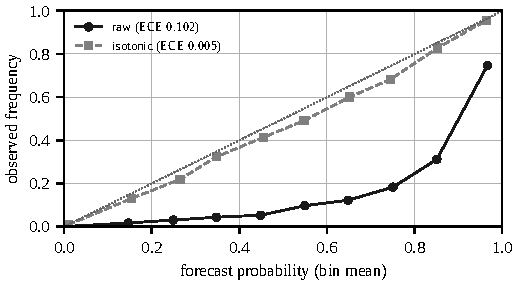
\includegraphics[width=0.9\columnwidth]{fig_rel.pdf}
\caption{Reliability of the forecast probabilities on the unseen test gauges, before and after isotonic recalibration fitted on validation data (bins with at least 50 gauge-days).}
\label{fig:rel}
\end{figure}

\begin{table}[t]
\caption{Operating points on the test set (threshold \Thr{} set on validation)}
\label{tab:ops}
\centering
\footnotesize
\begin{tabular}{cccc}
\toprule
Threshold & Recall & Precision & Alarms / 1000 days\\
\midrule
0.30 & 0.942 & 0.261 & 197.2\\
0.45 & 0.902 & 0.328 & 150.2\\
0.60 & 0.845 & 0.413 & 111.6\\
0.75 & 0.760 & 0.539 & 77.0\\
\bottomrule
\end{tabular}
\end{table}


Table~\ref{tab:warn} gives the lead of the warnings. The model warned three days ahead for \WarnThreeXgb\% of the \EvN{} onsets at \EvGauges{} gauges, with a mean lead of \MeanLeadXgb{} days when it warned. Climatology (\WarnThreeClim\%) and the LSTM simulation (\WarnThreeLstm\%) appear better on this measure, but for different reasons: climatology raises an alarm on most monsoon days, which its precision of \ClimPrec{} reflects, and the LSTM simulation is given the rain that is still to fall. Lead counts alone therefore reward methods that alarm constantly: random alarms at the model's average rate would warn of \RandWarn\% of onsets within three days, and at its monsoon rate of \RandWarnMon\%. Officers act on episodes rather than days; grouped into runs of consecutive alarm days, the model raised \EpN{} alarm episodes at the test gauges, of which \EpFalse{} (\EpFalsePct\%) contained no flood window.

\begin{table}[t]
\caption{Warning lead before the \EvN{} flood onsets (\% of onsets)}
\label{tab:warn}
\centering
\footnotesize
\setlength{\tabcolsep}{3pt}
\begin{tabular}{lccccc}
\toprule
Method & 3 days & 2 days & 1 day & none & Mean lead\\
\midrule
XGBoost (ours) & 63.9 & 16.5 & 10.9 & 8.6 & 2.58\\
No-flow XGB. & 72.2 & 14.7 & 7.1 & 6.0 & 2.69\\
LSTM sim.$^\dagger$ & 78.9 & 4.5 & 0.0 & 16.5 & 2.95\\
Climatology & 89.1 & 0.4 & 0.0 & 10.5 & 3.00\\
\bottomrule
\multicolumn{6}{l}{\scriptsize Mean lead in days, over warned onsets. $^\dagger$Driven by observed future rain.}\\
\end{tabular}
\end{table}

Skill was consistent across rivers: over the \PgN{} test gauges with at least one flood window, the median per-gauge balanced accuracy was \PgMed{} (interquartile range \PgQOne--\PgQThree), and the worst gauge reached \PgMin. For the \EvN{} flood onsets at the test gauges, the model warned one to three days ahead in \EvXgbWarn\% of cases, against \EvLstmWarn\% for the LSTM simulation, \EvClimWarn\% for climatology and \EvPersWarn\% for persistence, which by definition cannot anticipate an onset. The no-flow variant warned of \EvNoFlowWarn\%, more than the full model, but at a lower precision (\NoFlowPrec), and onset counts reward frequent alarms.

\subsection{Where the Forecast Succeeds and Fails}
\textit{Lead day.} The target pools three lead days, so we split the recall by the day on which the river is above its flood level. The model raised an alarm on day $t$ for \LeadOne\% of flood days at $t{+}1$, \LeadTwo\% at $t{+}2$ and \LeadThree\% at $t{+}3$. On rivers still below their flood level on day $t$, which is where a warning is useful, the rates were lower: \LeadOneRise\%, \LeadTwoRise\% and \LeadThreeRise\%.


\textit{Season.} Table~\ref{tab:season} separates the monsoon months. In June to September the model raised \MonAlarms{} alarms per 1,000 gauge-days at a precision of \MonPrec, against \OthAlarms{} and \OthPrec{} in the rest of the year, and \FpMonsoonPct\% of all false alarms fell in the monsoon. Most of these were not near misses: in the median monsoon false alarm the river peaked at \FaRatioMon\% of its flood level over the next three days, and only \NearMissMon\% of them reached 70--100\%. The model thus responds to monsoon conditions in general more than to an approaching flood.

\begin{table}[t]
\caption{Skill by season on the unseen test gauges}
\label{tab:season}
\centering
\footnotesize
\setlength{\tabcolsep}{2.6pt}
\begin{tabular}{lcccccc}
\toprule
Months & Gauge-days & Flood \% & BA & Rec. & Prec. & Alarms/1000\\
\midrule
Jun--Sep & 17,992 & 12.7 & 0.811 & 0.915 & 0.311 & 372\\
Oct--May & 35,002 & 1.8 & 0.918 & 0.857 & 0.415 & 36\\
\bottomrule
\end{tabular}
\end{table}

\textit{Catchment.} Over the \PgGauges{} test gauges with flood windows, per-gauge balanced accuracy rose with catchment area (Spearman $\rho=\RhoArea$, $p=\PArea$), which is consistent with large rivers rising slowly enough for today's flow to describe the next three days. Aridity, mean rainfall and slope showed no relation ($p\ge\PMinOther$). We expect, but have not tested, that rainfall forecasts would help most in small, fast catchments.


\section{Discussion and Limitations}
First, the inputs play different roles. Today's flow carries the overall score, while at flood onsets neither input group alone matched the full model, so an operations room needs both a reliable gauge feed and good meteorological inputs; when the feed fails, the no-flow variant scored above climatology. Second, precision is the weak point: most false alarms fell in June to September on rivers that stayed well below their flood level. The LSTM simulation, which is given the observed future rain, reached a precision of only \LstmPrec, so better rainfall information alone may not fix it. Until precision improves, an alarm should start a review, not an evacuation. Third, \LeakDiscuss{}


In deployment the full model would run while the gauge feed is live and the no-flow model when it is not, with recalibrated scores and officer review of every alarm; the fallback was evaluated offline only.

For studies that report flood forecasts on Indian rivers, the results suggest a minimal protocol: hold out both gauges and later years and report the split with the score (Table~\ref{tab:leak}); set flood thresholds, models and decision thresholds from training and validation years only; report precision and alarm rates by season (Table~\ref{tab:season}) and skill on onset rows (Table~\ref{tab:abl}); and check calibration before showing a score as a probability (Fig.~\ref{fig:rel}).

The study has limits. The CAMELS-IND gauges are in peninsular India, so skill may not transfer to Himalayan or Brahmaputra rivers. The 95th-percentile threshold is a statistical proxy for an official danger level. The LSTM reference was trained by the dataset authors on years and, most likely, gauges that overlap our test set, and it sees future rain, so the comparison with it is indicative only. We pool three lead days into one target. Intervals resample gauges but not years, and gauges in one monsoon share storms, so they are likely too narrow; skill per full test year ranged from \YearMinBA{} to \YearMaxBA, and was lower in the partial years \YearsSmall{} (\YearsSmallBA). The inputs other than rainfall come from reanalysis, so real-time skill will be lower. The ablation and protocol models were refitted on a 500,000-row sample, so they are compared with each other; the all-input refit scored \AblAllBA, as the selected model trained on all rows did (\XgbBA).

\section{Conclusion}
On CAMELS-IND gauges held out in space and time, a gradient-boosted model forecast three-day exceedance of the 95th-percentile flow with a balanced accuracy of \XgbBA{} and a PR-AUC of \XgbPR, above persistence and the gauge's own climatology, and comparable to the dataset's LSTM simulation, which sees future rain. Skill above persistence held across other gauge splits and whole held-out basins. On flood onsets the skill was lower (\OnXgbBA), not significantly different from the LSTM, and neither streamflow nor meteorological inputs alone matched the full model. Precision of \XgbPrec{}, lowest in the monsoon, and miscalibrated raw scores make the model a trigger for review by an officer, not an order. \LeakConclude{} Code and split lists will be released after review.

\section*{Acknowledgment}
The authors thank the CAMELS-IND and INDOFLOODS dataset authors for openly available data.
In line with the IEEE policy on AI-generated content, the authors disclose that Claude (Anthropic) was used to help edit and restructure the text of all sections and to draft the experiment and plotting scripts. All experiments use the authors' own software and fixed seeds. The authors checked every number, claim and reference and take full responsibility for the content.

\balance
\begin{thebibliography}{00}
\bibitem{Kratzert2019a} F. Kratzert, D. Klotz, G. Shalev, G. Klambauer, S. Hochreiter, and G. Nearing, ``Towards learning universal, regional, and local hydrological behaviors via machine learning applied to large-sample datasets,'' \textit{Hydrol. Earth Syst. Sci.}, vol. 23, pp. 5089--5110, 2019, doi: 10.5194/hess-23-5089-2019.
\bibitem{Kratzert2019b} F. Kratzert, D. Klotz, M. Herrnegger, A. K. Sampson, S. Hochreiter, and G. S. Nearing, ``Toward improved predictions in ungauged basins: Exploiting the power of machine learning,'' \textit{Water Resour. Res.}, vol. 55, pp. 11344--11354, 2019, doi: 10.1029/2019WR026065.
\bibitem{Nearing2024} G. Nearing \textit{et al.}, ``Global prediction of extreme floods in ungauged watersheds,'' \textit{Nature}, vol. 627, pp. 559--563, 2024, doi: 10.1038/s41586-024-07145-1.
\bibitem{Kapoor2023} S. Kapoor and A. Narayanan, ``Leakage and the reproducibility crisis in machine-learning-based science,'' \textit{Patterns}, vol. 4, no. 9, Art. no. 100804, 2023, doi: 10.1016/j.patter.2023.100804.
\bibitem{Roberts2017} D. R. Roberts \textit{et al.}, ``Cross-validation strategies for data with temporal, spatial, hierarchical, or phylogenetic structure,'' \textit{Ecography}, vol. 40, no. 8, pp. 913--929, 2017, doi: 10.1111/ecog.02881.
\bibitem{Mangukiya2025} N. K. Mangukiya \textit{et al.}, ``CAMELS-IND: Hydrometeorological time series and catchment attributes for 228 catchments in Peninsular India,'' \textit{Earth Syst. Sci. Data}, vol. 17, pp. 461--491, 2025, doi: 10.5194/essd-17-461-2025.
\bibitem{Newman2015} A. J. Newman \textit{et al.}, ``Development of a large-sample watershed-scale hydrometeorological data set for the contiguous USA: Data set characteristics and assessment of regional variability in hydrologic model performance,'' \textit{Hydrol. Earth Syst. Sci.}, vol. 19, pp. 209--223, 2015, doi: 10.5194/hess-19-209-2015.
\bibitem{Addor2017} N. Addor, A. J. Newman, N. Mizukami, and M. P. Clark, ``The CAMELS data set: Catchment attributes and meteorology for large-sample studies,'' \textit{Hydrol. Earth Syst. Sci.}, vol. 21, pp. 5293--5313, 2017, doi: 10.5194/hess-21-5293-2017.
\bibitem{Frame2022} J. M. Frame \textit{et al.}, ``Deep learning rainfall--runoff predictions of extreme events,'' \textit{Hydrol. Earth Syst. Sci.}, vol. 26, pp. 3377--3392, 2022, doi: 10.5194/hess-26-3377-2022.
\bibitem{Kirschstein2024} N. Kirschstein and Y. Sun, ``The merit of river network topology for neural flood forecasting,'' in \textit{Proc. 41st Int. Conf. Mach. Learn. (ICML)}, PMLR vol. 235, Vienna, Austria, 2024, pp. 24713--24725.
\bibitem{Alfieri2013} L. Alfieri \textit{et al.}, ``GloFAS -- global ensemble streamflow forecasting and flood early warning,'' \textit{Hydrol. Earth Syst. Sci.}, vol. 17, pp. 1161--1175, 2013, doi: 10.5194/hess-17-1161-2013.
\bibitem{Cloke2009} H. L. Cloke and F. Pappenberger, ``Ensemble flood forecasting: A review,'' \textit{J. Hydrol.}, vol. 375, pp. 613--626, 2009, doi: 10.1016/j.jhydrol.2009.06.005.
\bibitem{Nevo2022} S. Nevo \textit{et al.}, ``Flood forecasting with machine learning models in an operational framework,'' \textit{Hydrol. Earth Syst. Sci.}, vol. 26, no. 15, pp. 4013--4032, 2022, doi: 10.5194/hess-26-4013-2022.
\bibitem{Kuntla2025} S. K. Kuntla and M. Saharia, ``INDOFLOODS: A comprehensive database for flood events in India enhanced with catchment attributes,'' \textit{Bull. Amer. Meteorol. Soc.}, vol. 106, no. 2, pp. E333--E343, 2025, doi: 10.1175/BAMS-D-24-0008.1.
\bibitem{Mosavi2018} A. Mosavi, P. Ozturk, and K.-W. Chau, ``Flood prediction using machine learning models: Literature review,'' \textit{Water}, vol. 10, no. 11, Art. no. 1536, 2018, doi: 10.3390/w10111536.
\bibitem{Saito2015} T. Saito and M. Rehmsmeier, ``The precision-recall plot is more informative than the ROC plot when evaluating binary classifiers on imbalanced datasets,'' \textit{PLoS ONE}, vol. 10, no. 3, Art. no. e0118432, 2015, doi: 10.1371/journal.pone.0118432.
\bibitem{Brier1950} G. W. Brier, ``Verification of forecasts expressed in terms of probability,'' \textit{Mon. Weather Rev.}, vol. 78, no. 1, pp. 1--3, 1950, doi: 10.1175/1520-0493(1950)078\textless{}0001:VOFEIT\textgreater{}2.0.CO;2.
\bibitem{Chen2016} T. Chen and C. Guestrin, ``XGBoost: A scalable tree boosting system,'' in \textit{Proc. 22nd ACM SIGKDD Int. Conf. Knowl. Discov. Data Min.}, 2016, pp. 785--794, doi: 10.1145/2939672.2939785.
\end{thebibliography}

\end{document}
